%\newcommand{\ein}[2]{(#1) (#2 Punkte)}
%\section*{\hfil Aufgaben \hfil}

\begin{Large}
\textbf{Teil I: Offene Fragen (36 Punkte)}
\end{Large}
\\
\\
\\
\textbf{Allgemeine Anweisungen für offene Fragen:}
\\
\renewcommand{\labelenumi}{(\roman{enumi})}
\begin{enumerate}
\item
Ihre Antworten müssen alle Rechenschritte enthalten,
diese müssen klar ersichtlich sein.
Verwendung korrekter mathematischer Notation wird erwartet
und fliesst in die Bewertung ein.

\item
Ihre Antworten zu den jeweiligen Teilaufgaben müssen in den dafür vorgesehenen Platz geschrie-
ben werden. Sollte dieser Platz nicht ausreichen, setzen Sie Ihre Antwort auf der Rückseite oder
dem separat zur Verfügung gestellten Papier fort. Verweisen Sie in solchen Fällen ausdrücklich
auf Ihre Fortsetzung. Bitte schreiben Sie zudem Ihren Vor- und Nachnamen auf jeden separaten
Lösungsbogen.

\item
Es werden nur Antworten im dafür vorgesehenen Platz bewertet. Antworten auf der Rückseite
oder separatem Papier werden nur bei einem vorhandenen und klaren Verweis darauf bewertet.

\item
Die Teilaufgaben werden mit den jeweils oben auf der Seite angegebenen Punkten bewertet.

\item
Ihre endgültige Lösung jeder Teilaufgabe darf nur eine einzige Version enthalten.

\item
Zwischenrechnungen und Notizen müssen auf einem getrennten Blatt gemacht werden. Diese
Blätter müssen, deutlich als Entwurf gekennzeichnet, ebenfalls abgegeben werden.
\end{enumerate}

\newpage

\vspace{1cm}
\section*{Aufgabe 1 (36 Punkte)}
\vspace{0.4cm}
\subsection*{\aufgabe{a1}{6}}
Für Preise $ p \in [0,3] $ kann der Markt für ein bestimmtes Gut beschrieben werden durch die Angebotsfunktion
\begin{align*}
q_s : \mathbb{R}_+ \to \mathbb{R}, p \mapsto q_s(p)= 4 e^{p-1}
\end{align*}
und die Nachfragefunktion 
\begin{align*}
q_d: \mathbb{R}_+ \to \mathbb{R}, p \mapsto q_d(p) = 70 -15p -1.5p^2.
\end{align*}
Beweisen Sie: Es gibt genau ein Marktgleichgewicht $ (p^\star,q^\star) $ mit Gleichgewichtspreis $ p^\star \in [2,3]$ und Gleichgewichtsmenge $ q^\star \in \mathbb{R}_+ $.
\\
\\
\subsection*{\aufgabe{a2}{6}}
Für Preise $ p \in [0,3] $ kann der Markt für ein bestimmtes Gut beschrieben werden durch die Angebotsfunktion
\begin{align*}
q_s : \mathbb{R}_+ \to \mathbb{R}, p \mapsto q_s(p) 4 e^{p-1}
\end{align*}
und die Nachfragefunktion 
\begin{align*}
q_d: \mathbb{R}_+ \to \mathbb{R}, p \mapsto q_d(p) = 70 -15p -1.5p^2.
\end{align*}
Der Markt hat genau ein Marktgleichgewicht $ (p^\star,q^\star) $ mit $ p^\star \in [2,3] $.\\
Berechnen Sie $ p^\star  $ näherungsweise mit Hilfe eines Taylorpolynoms 2. Ordnung in $ p_0 = 1 $.

\subsection*{\aufgabe{b}{10}}
Nina entschliesst sich am Anfang des Jahres, in dem sie ihr Studium beginnt, einen Studienkredit
von CHF $ 100'000 $ aufzunehmen. Sie tut dies trotz des hohen Zinssatzes von $ i = 8 \% $, weil
vertragsgemäss die Zahlung der Zinsen und die Rückzahlung erst im Jahr nach Abschluss ihres
Studiums beginnt.
Dann sollen der Kredit und die Zinsen in $ 10  $ gleichmässigen Raten $ C $, jeweils am Jahresende bezahlt werden.\\
Nina schliesst ihr Studium nach $ 5\frac{1}{2} $ Jahren ab. (\textit{Hinweis: Sie hat damit noch $ 18  $ Monate, bis die erste Rate fällig wird.})
\begin{enumerate}
	\item[(b1)]
	Zeichnen Sie die beschriebenen Zahlungsströme und Ereignisse an einem Zeitstrahl an.
	\item[(b2)] 
	Wie hoch sind Nina's Schulden zu Beginn des Jahres in dem die Rückzahlung beginnt?
	\item[(b3)] 
	Bestimmen Sie die Höhe der vereinbarten Raten $ C $.
\end{enumerate}
Nachdem sie schon $ 5 $ Raten abbezahlt hat, macht Nina eine Erbschaft von CHF $ 100'000 $.
Sie beschliesst, statt der $ 6. $ Rate den ganzen Restbetrag zurückzuzahlen.
\begin{enumerate}
	\item[(b4)] 
	Ergänzen Sie die Info am Zeitstrahl.
	\item[(b5)] 
	Reichen die CHF $ 100'000 $, um die Schulden vollkommen zurückzuzahlen?\\
	Wenn ja: Wie viel bleibt Nina von ihrer Erbschaft?\\
	Wenn nein: Welchen zusätzlichen Betrag muss Nina zur Tilgung ihrer Schulden aufbringen?
\end{enumerate}

\subsection*{\aufgabe{c}{5}}
Im Jahre 1955 entwickelte Morris Swadesh (1909-1967) eine (umstrittene) Methode, die sog.
Glottochronologie, um den Zeitpunkt zu bestimmen, an dem zwei verwandte Sprachen (z. B.
Latein und Sanskrit) sich verzweigten. Swadesh ging von der Hypothese aus, dass die sprachlichen
Atome - d.h. die Wörter - zerfallen wie radioaktive Atome. Laut Voraussetzung soll der
grundlegende Urwortschatz der Sprachen mit einer Halbwertszeit von etwa 2000 Jahren aussterben.
Kennt man die Menge des noch gemeinsamen Urwortschatzes zweier Sprachen und geht
davon aus, dass sich diese Menge alle 2000 Jahre halbiert, kann man berechnen, wann sich
die Sprachen verzweigt haben. A. Raun und E. Kangsmaa-Minn führten unabhänging voneinander,
d.h. jeweils mit einer eigenen Methode, den Vergleich des Finnischen und Ungarischen
durch. Während Raun herausfand, dass der Anteil der identischen Elemente in beiden Sprachen
$21 \% $ beträgt, berechnete Kangsmaa-Minn einen Anteil von $ 27 \% $.\\
Innerhalb welches Zeitraums haben sich die beiden Sprachen nach der Theorie der Glottochronolgie
und aufgrund dieser Zahlen voneinander getrennt?\\
\\
\textit{Bemerkung}:\\
Berechnen Sie also, vor wie vielen Jahren sich das Finnische und das Ungarische gemäss a)
der Berechnung von A. Raun und b) der Berechnung von E. Kangsmaa-Minn getrennt haben.
Geben Sie das finale Ergebnis als Zeitintervall an.\\
\\
\subsection*{\aufgabe{d}{9}}
Ein Student hat ein gegenwärtiges Einkommen von CHF $ 3'000 $ und erwartet in einem Jahr ein zukünftiges Einkommen von CHF $ 7'000 $. Er plant einen gegenwärtigen Konsum $ c_1 $ und im
folgenden Jahr einen Konsum $ c_2 $ mit der Absicht die Nutzenfunktion $ u = \ln(c_1) + \frac{1}{1.2}
\ln(c_2) $ zu maximieren.\\
Wenn er jetzt Geld leiht, weil $ c_1 > 3'000 $ CHF ist, dann wird der zukünftige Konsum $ c_2 $ nach
Rückzahlung des Kreditbetrages und der Zinsen berechnet. Spart er entsprechend Geld, i. e.
$ c_1 < 3'000 $ CHF, dann kann er $ c_2 $ um den gesparten Betrag und dessen Zinsen erhöhen. Der (optimistische)
Zinssatz für Leihen und Sparen beträgt $ i = 8\% $.
\begin{enumerate}
	\item[(d1)] Bestimmen Sie den Zusammenhang zwischen $ c_1 $ und $ c_2 $.
	\item[(d2)] Bestimmen Sie den Nutzen des Studenten in Abhängigkeit von $ c_1 $.
	\item[(d3)] Für welche Wahl von $ c_1 $ ist der Nutzen des Studenten maximal?\\
	Wie viel muss er sich allenfalls leihen? 
\end{enumerate}
\newpage
\fancyhead[C]{\normalsize\textbf{$\qquad$ Teil II: Multiple-Choice}}
\begin{Large}
\textbf{Teil II: Multiple-Choice-Fragen (64 Punkte)}
\end{Large}
\\
\\
\\
\textbf{Allgemeine Anweisungen für Multiple-Choice-Fragen:}
\\
\renewcommand{\labelenumi}{(\roman{enumi})}
\begin{enumerate}
\item
Die Antworten auf die Multiple-Choice-Fragen müssen im dafür vorgesehenen Antwortbogen ein-
getragen werden. Es werden ausschliesslich Antworten auf diesem Antwortbogen bewertet. Der
Platz unter den Fragen ist nur für Notizen vorgesehen und wird nicht korrigiert.

\item
Jede Frage hat nur eine richtige Antwort. Es muss also auch jeweils nur eine Antwort angekreuzt
werden.

\item
Falls mehrere Antworten angekreuzt sind, wird die Antwort mit 0 Punkten bewertet, auch wenn
die korrekte Antwort unter den angekreuzten ist.

\item
Bitte lesen Sie die Fragen sorgfältig.

\end{enumerate}
\newpage
\section*{Aufgabe 2 (34 Punkte)}
\vspace{0.4cm}
\subsection*{\frage{1}{2}}
Die Aussage \glqq Wenn Albert kommt, dann kommt auch Beatrice\grqq~sei richtig.
Dann ist die folgende Aussage sicher auch richtig:
\renewcommand{\labelenumi}{(\alph{enumi})}
\begin{enumerate}
	\item \glqq Wenn Beatrice kommt, dann kommt auch Albert\grqq
	\item \glqq Wenn Albert nicht kommt, dann kommt auch Beatrice nicht\grqq
	\item
	\glqq Wenn Beatrice nicht kommt, dann kommt auch Albert nicht\grqq
	
	\item
	Keine der Aussagen (a)-(c) ist sicher richtig.
\end{enumerate}
\ \\
\subsection*{\frage{2}{2}}
Die Folge $ \lbrace a_n \rbrace_{n \in \mathbb{N}} $ ist monoton wachsend und beschränkt. Die Folge $ \lbrace b_n \rbrace_{n \in \mathbb{N} }  $ ist definiert durch $ b_n = 2 a_n -1 $.\\
Dann ist $ \lbrace b_n \rbrace_{n \in \mathbb{N}} $
\renewcommand{\labelenumi}{(\alph{enumi})}
\begin{enumerate}
\item konvergent.
\item divergent.
\item
monoton fallend.
\item
unbeschränkt.
\end{enumerate}
\ \\
\subsection*{\frage{3}{3}}
Ein Kapital von $ P = 1'000'000 $ CHF wird angelegt bei einem Jahreszinssatz von $ i = 2\% $ mit monatlicher Verzinsung.\\
Der effektive Zinssatz $ i_{\textrm{eff}} $ beträgt näherungsweise 
\renewcommand{\labelenumi}{(\alph{enumi})}
\begin{enumerate}
\item 
$ 1.982 \% $.
\item 
$ 2 \% $.
\item 
$ 2.018 \% $.
\item
$ 2.020 \% $.
\end{enumerate}
\ \\
\subsection*{\frage{4}{3}}
Die Funktion $ f $ ist gegeben durch
\begin{align*}
f : D_f \to \mathbb{R}, \ 
x \mapsto y = f(x) = - \frac{3}{x^5} +2
\end{align*}
Dann ist die inverse Funktion $ f^{-1} $ definiert auf 
\renewcommand{\labelenumi}{(\alph{enumi})}
\begin{enumerate}
\item 
$ \mathbb{R} $.
\item
$ \mathbb{R} \setminus \lbrace 0 \rbrace $.
\item
$ \mathbb{R} \setminus \lbrace 2 \rbrace $.
\item
Die Funktion $ f $ ist nicht injektiv. Deshalb ist es unmöglich, eine Umkehrfunktion $ f^{-1} $ anzugeben.
\end{enumerate}
\ \\
\subsection*{\frage{5}{4}}
Seien $ m,n,k > 0 $, $ m \neq 1 $, $ n \neq 1 $, $ k \neq 1 $.\\
Welche der folgenden Identitäten ist allgemein gültig?
\renewcommand{\labelenumi}{(\alph{enumi})}
\begin{enumerate}
\item 
$ n^{\log_m(k)} = k^{\log_n(m)} $.
\item
$ n^{\log_m(k)} = k^{\log_m(n)}$.
\item
$ n^{\log_m(k)} = m^{\log_n(k)}$.
\item
Keine der Identitäten (a) - (c) gilt allgemein.
\end{enumerate}
\ \\ 
\subsection*{\frage{6}{3}}
Wir betrachten die Funktion
\begin{align*}
f(x) = \frac{1}{(\sin(x))^2}- 2 \pi, -2 \pi < x < 2 \pi.
\end{align*}

Welche der folgenden Behauptungen ist wahr?
\renewcommand{\labelenumi}{(\alph{enumi})}
\begin{enumerate}
\item 
$ f $ ist stetig für alle $ x \in (-2 \pi, 2 \pi) \setminus \lbrace 0 \rbrace $.
\item
$ f $ hat mehr als eine Unstetigkeitsstelle in $ (- 2 \pi , 2 \pi ) $.

\item
$ f $ ist überall stetig.
\item
$ f $ hat keine Polstelle.
\end{enumerate}
\ \\
\subsection*{\frage{7}{3}}
Gegeben ist die Funktion $ f $ durch
\begin{align*}
f : D_f \to \mathbb{R}, \ x \mapsto y = f(x) = \frac{x}{3} - \frac{e}{x^3}.
\end{align*}
Der Wertebereich von $ f^\prime$ ist
\renewcommand{\labelenumi}{(\alph{enumi})}
\begin{enumerate}
\item 
$ (- \infty,0) \cup (0,\infty) $.
\item
$ (-\infty,\infty) $.
\item
$ (0, \infty) $
\item
$ ( \frac{1}{3}, \infty) $
\end{enumerate}
\ \\
\subsection*{\frage{8}{3}}
Gegeben ist eine differenzierbare Funktion $ f $ mit Ableitung $ f^\prime $.\\
Welche der folgenden Aussagen ist falsch?
\renewcommand{\labelenumi}{(\alph{enumi})}
\begin{enumerate}
\item 
$ f  $ ist stetig.
\item
Wenn $ f $ gerade ist, dann ist auch $ f^\prime $ gerade.
\item
Wenn $ f $ gerade ist, dann ist $ f^\prime $ ungerade.
\item
Wenn $ f^\prime > 0 $ ist, dann ist $ f $ streng monoton wachsend.
\end{enumerate}
\ \\
\subsection*{\frage{9}{3}}
Für eine differenzierbare Funktion $ h:D_h \to \mathbb{R}, x \mapsto y = h(x) $ seid $ dh(x) $ ihr Differential an der Stelle $ x $.
Wir betrachten nun zwei differenzierbare Funktionen $ f :D_f \to \mathbb{R} $ und $ g: D_g \to \mathbb{R} $ und Konstanten $ a,b \in \mathbb{R} $.\\
Welche der folgenden Gleichungen ist im Allgemeinen falsch?
\renewcommand{\labelenumi}{(\alph{enumi})}
\begin{enumerate}
	\item 
	$ d(af +bg)(x) = a \ df(x) + b \ d g(x) $.
	\item
	$ d(fg)(x) = g(x) \ df(x) + f(x) \ dg(x) $.
	\item
	$ d(f\circ g) (x) = f^\prime(g(x)) \ dg(x) $.
	\item
	$ d \left( \frac{f}{g} \right)(x) = g(x) \ df(x) - f(x) \ dg(x) $.
\end{enumerate}

\subsection*{\frage{10}{3}}
Wir betrachten die Funktion
\begin{align*}
f : D_f \to \mathbb{R}, \ x \mapsto y = f(x) = | x^2 - 2x -24 |.
\end{align*}
Welche der folgenden Behauptungen ist wahr?
\renewcommand{\labelenumi}{(\alph{enumi})}
\begin{enumerate}
	\item 
	$ f $ hat ein lokales Maximum in $ x_0 = 1 $.
	\item
	$ f $ hat ein globales Maximum in $ x_0 = 1 $.
	\item
	$ f  $ hat ein eindeutiges globales Maximum.
	\item
	$ f $ hat ein eindeutiges lokales Minimum.
\end{enumerate}
\ \\
\subsection*{\frage{11}{3}}
Sei 
\begin{align*}
P(x) = 1 + 2x + 5x^2 -x^3
\end{align*}
des Taylor-Polynoms 3. Ordnung an der Stelle $ x_0 = 0 $ einer unendliche oft differenzierbaren Funktion $ f $.\\
Welche der folgenden Aussagen sind korrekt?
\renewcommand{\labelenumi}{(\alph{enumi})}
\begin{enumerate}
	\item 
	$ f(0) = 2 $.
	\item
	$ f^\prime(0) = 1 $.
	\item
	$ f^{\prime \prime}(0) = 10 $.
	\item
	$ f^{(3)}(0) = -5 $.
\end{enumerate}
\ \\
\subsection*{\frage{12}{2}}
Eine homogene Funktion $ f $ hat den Grad $ 1.8 $.
Ausserdem kennt man die partielle Elastizität
$ \varepsilon_{f,y}(x,y) = x +y -1.2 $.\\
Es folgt dann 
\renewcommand{\labelenumi}{(\alph{enumi})}
\begin{enumerate}
	\item 
	$ \varepsilon_{f,x}(x,y) = x-y -1.2 $.
	\item
	$ \varepsilon_{f,x}(x,y) = -x-y +1.2 $.
	\item
	$ \varepsilon_{f,x}(x,y) = -x-y +3 $.
	\item
	$ \varepsilon_{f,x}(x,y) $ ist durch die Angaben nicht eindeutig bestimmt.
\end{enumerate}

\newpage
\section*{Aufgabe 3 (30 Punkte)}
\vspace{0.4cm}

\subsection*{\frage{1}{4}}
Der  Grenzwert
\begin{align*}
\lim \limits_{x\to 0} 
\frac{e^x + e^{-x} -2}{1 - \cos(x)}
\end{align*}
ist
\renewcommand{\labelenumi}{(\alph{enumi})}
\begin{enumerate}
\item 
$ 0 $.
\item
$ 0.5 $.
\item
$ 1 $.
\item
$ 2 $.
\end{enumerate}
\ \\
\subsection*{\frage{2}{4}}
Der Grenzwert
\begin{align*}
\lim \limits_{x \to 3} 
\left(\frac{1}{x-3} - \frac{27}{x^3 - 27}\right)
\end{align*}
ist
\renewcommand{\labelenumi}{(\alph{enumi})}
\begin{enumerate}
\item 
$ 0 $.
\item
$ \frac{1}{3} $.
\item
$ \frac{2}{5} $.
\item
$ \infty $.
\end{enumerate}
\ \\
\subsection*{\frage{3}{4}}
Am $ 26.12.2017 $ entdeckte der Hobby-Mathematiker Jonathan Price aus Germantown, Tennessee, die bislang grösste bekannte Primzahl $ p $, nämlich
\begin{align*}
p = 2^{77'232'917} -1
\end{align*}
Wie viele Stellen hat $ p $ im Dezimalsystem?\\
(\textit{Tipp:} Überlegen Sie sich den Zusammenhang zwischen Anzahl Stellen einer natürlichen Zahl $ n $ im Dezimalsystem und ihrem Zehnerlogarithmus $ \log_{10}(n) $) 
\renewcommand{\labelenumi}{(\alph{enumi})}
\begin{enumerate}
\item 
$ p $ hat im Dezimalsystem $ 23'249'424 $ Stellen.
\item
$ p $ hat im Dezimalsystem $ 23'249'425 $ Stellen.
\item
$ p $ hat im Dezimalsystem $ 53'533'778 $ Stellen.
\item
$ p $ hat im Dezimalsystem $ 53'533'779 $ Stellen.
\end{enumerate}
\ \\
\subsection*{\frage{4}{3}}
Gegeben sei die Funktion in zwei reellen Variablen
\begin{align*}
f : D_f \to \mathbb{R}, (x,y) \mapsto
z = f(x,y) = \sqrt[4]{4x^2 + 4 y^2 - 36}
+ \frac{1}{\sqrt{x^2 - y -2}}.
\end{align*}
Welches der folgenden Bilder zeigt grau schraffiert den Definitionsbereich $ D_f \subset \mathbb{R}^2 $ von $ f $?
\renewcommand{\labelenumi}{(\alph{enumi})}
\begin{center}
	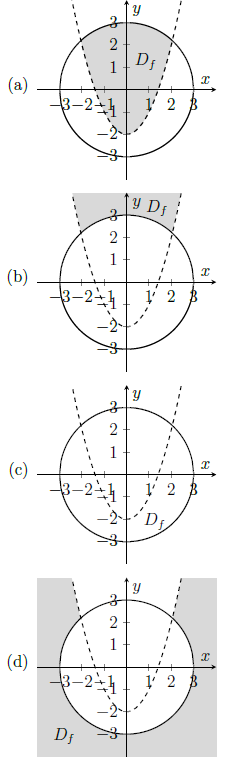
\includegraphics{pictures/auf3_4}
\end{center}

\newpage
\subsection*{\frage{5}{4}}
Betrachte die Funktion
\begin{align*}
f : D_f \to \mathbb{R}, 
(x,y) \mapsto z = f(x,y) = \ln(\sqrt{e} -x^2 -y^2)
\end{align*}
mit dem Definitionsbereich
\begin{align*}
D_f
= \{
(x,y) \in \mathbb{R}^2 : x^2 + y^2 \leq \sqrt{e}
\}.
\end{align*}
Dann ist das Bild $ R_f $ von $ f $ gegeben durch
\renewcommand{\labelenumi}{(\alph{enumi})}
\begin{enumerate}
\item 
$R_f = \mathbb{R} $.
\item
$R_f = \left( -\frac{1}{2}, \frac{1}{2} \right) $.
\item
$R_f = \left(  \frac{1}{2}, \infty \right) $.
\item
$R_f = \left( -\infty, \frac{1}{2} \right) $.
\end{enumerate}
\ \\
\subsection*{\frage{6}{4}}
Betrachte die Funktion
\begin{align*}
f :D_f \to \mathbb{R},
(x,y) \mapsto
z = f(x,y) = \ln \left( \left| \frac{y+1}{x-2} \right|\right).
\end{align*}
Die Steigung $ m $ der Tangenten an die Niveaulinie $ f(x,y) = \ln(2) $ im Punkt $ (x_0,y_0) = (1,1) $ ist gegeben durch
\renewcommand{\labelenumi}{(\alph{enumi})}
\begin{enumerate}
\item 
$ m = -0.5 $.
\item
$ m = 0.5 $.
\item
$ m = -2 $.
\item
Es ist nicht möglich, die Steigung $ m $ als Funktion von $ x $ anzugeben.
\end{enumerate}
\ \\
\subsection*{\frage{7}{3}}
Gegeben sind die Funktionen
\begin{align*}
f(x,y) =  \ln
\left( x^2 \sqrt{y} + \sqrt[4]{x^3 y^7}\right) - \frac{5}{2} \ln(x).
\end{align*}
wobei $ x> 0 $, $ y >0  $.
\renewcommand{\labelenumi}{(\alph{enumi})}
\begin{enumerate}
\item
$ f $ ist homogen vom Grad $ 0 $.

\item 
$ f $ ist linear homogen.
\item
$ f $ ist homogen vom Grad $ \frac{5}{2} $.
\item
$ f $ ist nicht homogen.
\end{enumerate}
\ \\
\subsection*{\frage{8}{4}}
Gegeben sei die Funktion
\begin{align*}
f(x,y) = 
7x\sqrt{y^a} + 3y^2 \sqrt[4]{x^a y^b} - x^2 y^{0.2},
\end{align*}
wobei $ x > 0 $, $ y > 0 $ und $ a,b \in \mathbb{R} $.\\
Für welche Werte von $ a $ und $ b $ ist $ f  $ homogen?
\renewcommand{\labelenumi}{(\alph{enumi})}
\begin{enumerate}
\item 
$a = 2.4$, $ b = -2 $.
\item
$a = 2.4$, $ b = -1.6 $.
\item
$a = 2$, $ b = -1.2 $.
\item
$ f  $ ist homogen für alle $ a,b \in \mathbb{R} $.
\end{enumerate}